% questions.tex —— 2008 年·普通高等学校招生考试·江西卷·文科 · 题目内容片段（无答案）
% 由 tools/generate_projects.py 依来源总账自 2008/2008_数学真题_江西文_试题.md 生成，勿手改（改源 MD 后重跑）


\gkpart{一、选择题}

\begin{question}
\gkti{1}“$|x|=|y|$”是“$x=y$”的（　）

（A）充分不必要条件

（B）必要不充分条件

（C）充要条件

（D）既不充分也不必要条件

\end{question}
\begin{question}
\gkti{2}定义集合运算：$A*B=\{z\mid z=xy,\ x\in A,\ y\in B\}$。设 $A=\{1,2\}$，$B=\{0,2\}$，则集合 $A*B$ 的所有元素之和为（　）

（A）$0$

（B）$2$

（C）$3$

（D）$6$

\end{question}
\begin{question}
\gkti{3}若函数 $y=f(x)$ 的定义域是 $[0,2]$，则函数 $g(x)=\dfrac{f(2x)}{x-1}$ 的定义域是（　）

（A）$[0,1]$

（B）$[0,1)$

（C）$[0,1)\cup(1,4]$

（D）$(0,1)$

\end{question}
\begin{question}
\gkti{4}若 $0<x<y<1$，则（　）

（A）$3^y<3^x$

（B）$\log_x3<\log_y3$

（C）$\log_4x<\log_4y$

（D）$\left(\dfrac14\right)^x<\left(\dfrac14\right)^y$

\end{question}
\begin{question}
\gkti{5}在数列 $\{a_n\}$ 中，$a_1=2$，$a_{n+1}=a_n+\ln\left(1+\dfrac1n\right)$，则 $a_n=$（　）

（A）$2+\ln n$

（B）$2+(n-1)\ln n$

（C）$2+n\ln n$

（D）$1+n+\ln n$

\end{question}
\begin{question}
\gkti{6}函数 $f(x)=\dfrac{\sin x}{\sin x+2\sin\dfrac x2}$ 是（　）

（A）以 $4\pi$ 为周期的偶函数

（B）以 $2\pi$ 为周期的奇函数

（C）以 $2\pi$ 为周期的偶函数

（D）以 $4\pi$ 为周期的奇函数

\end{question}
\begin{question}
\gkti{7}已知 $F_1$、$F_2$ 是椭圆的两个焦点，满足 $\overrightarrow{MF_1}\cdot\overrightarrow{MF_2}=0$ 的点 $M$ 总在椭圆内部，则椭圆离心率的取值范围是（　）

（A）$(0,1)$

（B）$\left(0,\dfrac12\right]$

（C）$\left(0,\dfrac{\sqrt2}2\right)$

（D）$\left[\dfrac{\sqrt2}2,1\right)$

\end{question}
\begin{question}
\gkti{8}$(1+x)^{10}\left(1+\dfrac1x\right)^{10}$ 展开式中的常数项为（　）

（A）$1$

（B）$(\mathrm C_{10}^1)^2$

（C）$\mathrm C_{20}^1$

（D）$\mathrm C_{20}^{10}$

\end{question}
\begin{question}
\gkti{9}设直线 $m$ 与平面 $\alpha$ 相交但不垂直，则下列说法中正确的是（　）

（A）在平面 $\alpha$ 内有且只有一条直线与直线 $m$ 垂直

（B）过直线 $m$ 有且只有一个平面与平面 $\alpha$ 垂直

（C）与直线 $m$ 垂直的直线不可能与平面 $\alpha$ 平行

（D）与直线 $m$ 平行的平面不可能与平面 $\alpha$ 垂直

\Needspace{0.4\textheight}
\end{question}
\begin{question}
\gkti{10}函数 $y=\tan x+\sin x-|\tan x-\sin x|$ 在区间 $\left(\dfrac{\pi}2,\dfrac{3\pi}2\right)$ 内的图象大致是（　）
\nopagebreak[4]
\begin{center}% 2008 年江西卷文科第 10 题：y=tan x+sin x-|tan x-sin x| 在 (π/2,3π/2) 内的四个候选图象。
% 来源 PDF：gaokaomath-src/普通高考/2008/2008江西文.pdf
% SHA-256：8505b08b95152dbb1421e3f2d72c379b24c8ab6cb47bcc1dbdc8feb058459cda
% 原页：2008江西文.pdf 第 1 页（A3 三栏）第 2 栏，书页码 461。
% 绘制依据：由 |tan x - sin x| 分段，x∈(π/2,π) 时 y=2tan x（负值升到 0），
%   x∈(π,3π/2) 时 y=2sin x（由 0 降到 -2）。四个候选按原页 2×2 排布，
%   坐标刻度取 π/2→1、π→2、3π/2→3（单位长度相同），π/2 与 3π/2 的标号用白底压住虚线。
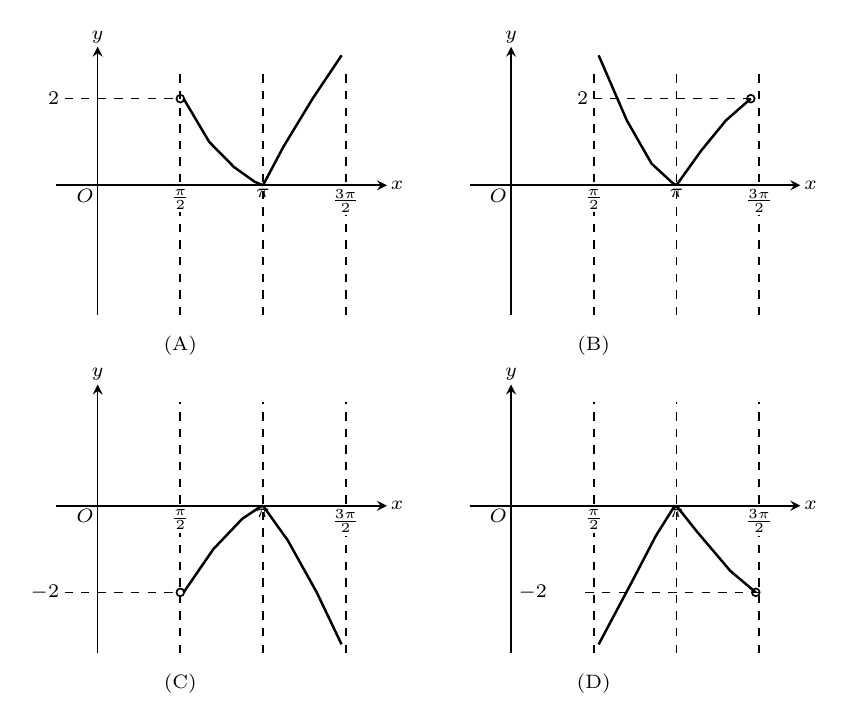
\begin{tikzpicture}[x=1.05cm, y=0.55cm, semithick, font=\scriptsize,
  every node/.style={inner sep=1.1pt}]

  % ---------- (A) ----------
  \begin{scope}[shift={(0,0)}]
    \draw[->,>=stealth] (-0.5,0) -- (3.5,0) node[right] {$x$};
    \draw[->,>=stealth] (0,-3.0) -- (0,3.2) node[above] {$y$};
    \node[below left] at (0,0) {$O$};
    \draw[dashed] (1.0,-3.0) -- (1.0,2.6);
    \draw[dashed] (2.0,-3.0) -- (2.0,2.6);
    \draw[dashed] (3.0,-3.0) -- (3.0,2.6);
    \node[below, fill=white] at (1.0,0) {$\frac{\pi}{2}$};
    \node[below] at (2.0,0) {$\pi$};
    \node[below, fill=white] at (3.0,0) {$\frac{3\pi}{2}$};
    \draw[dashed] (-0.4,2.0) -- (1.0,2.0);
    \node[left] at (-0.42,2.0) {$2$};
    \draw (1.0,2.0) circle (1.4pt);
    \draw[line width=0.9pt] plot coordinates {(1.04,2.0) (1.35,1.0) (1.65,0.42) (1.9,0.08) (2.0,0.0)};
    \draw[line width=0.9pt] plot coordinates {(2.0,0.0) (2.25,0.9) (2.6,2.0) (2.95,3.0)};
    \node at (1.0,-3.7) {(A)};
  \end{scope}

  % ---------- (B) ----------
  \begin{scope}[shift={(5.0,0)}]
    \draw[->,>=stealth] (-0.5,0) -- (3.5,0) node[right] {$x$};
    \draw[->,>=stealth] (0,-3.0) -- (0,3.2) node[above] {$y$};
    \node[below left] at (0,0) {$O$};
    \draw[dashed] (1.0,-3.0) -- (1.0,2.6);
    \draw[dashed] (2.0,-3.0) -- (2.0,2.6);
    \draw[dashed] (3.0,-3.0) -- (3.0,2.6);
    \node[below, fill=white] at (1.0,0) {$\frac{\pi}{2}$};
    \node[below] at (2.0,0) {$\pi$};
    \node[below, fill=white] at (3.0,0) {$\frac{3\pi}{2}$};
    \draw[dashed] (1.0,2.0) -- (2.9,2.0);
    \node[left] at (0.98,2.0) {$2$};
    \draw[line width=0.9pt] plot coordinates {(1.06,3.0) (1.4,1.5) (1.7,0.5) (1.95,0.06) (2.0,0.0)};
    \draw[line width=0.9pt] plot coordinates {(2.0,0.0) (2.3,0.8) (2.6,1.5) (2.9,2.0)};
    \draw (2.9,2.0) circle (1.4pt);
    \node at (1.0,-3.7) {(B)};
  \end{scope}

  % ---------- (C) ----------
  \begin{scope}[shift={(0,-7.4)}]
    \draw[->,>=stealth] (-0.5,0) -- (3.5,0) node[right] {$x$};
    \draw[->,>=stealth] (0,-3.4) -- (0,2.8) node[above] {$y$};
    \node[below left] at (0,0) {$O$};
    \draw[dashed] (1.0,-3.4) -- (1.0,2.4);
    \draw[dashed] (2.0,-3.4) -- (2.0,2.4);
    \draw[dashed] (3.0,-3.4) -- (3.0,2.4);
    \node[below, fill=white] at (1.0,0) {$\frac{\pi}{2}$};
    \node[below] at (2.0,0) {$\pi$};
    \node[below, fill=white] at (3.0,0) {$\frac{3\pi}{2}$};
    \draw[dashed] (-0.4,-2.0) -- (1.0,-2.0);
    \node[left] at (-0.42,-2.0) {$-2$};
    \draw (1.0,-2.0) circle (1.4pt);
    \draw[line width=0.9pt] plot coordinates {(1.04,-2.0) (1.4,-1.0) (1.75,-0.3) (1.97,-0.02) (2.0,0.0)};
    \draw[line width=0.9pt] plot coordinates {(2.0,0.0) (2.3,-0.8) (2.65,-2.0) (2.95,-3.2)};
    \node at (1.0,-4.1) {(C)};
  \end{scope}

  % ---------- (D) ----------
  \begin{scope}[shift={(5.0,-7.4)}]
    \draw[->,>=stealth] (-0.5,0) -- (3.5,0) node[right] {$x$};
    \draw[->,>=stealth] (0,-3.4) -- (0,2.8) node[above] {$y$};
    \node[below left] at (0,0) {$O$};
    \draw[dashed] (1.0,-3.4) -- (1.0,2.4);
    \draw[dashed] (2.0,-3.4) -- (2.0,2.4);
    \draw[dashed] (3.0,-3.4) -- (3.0,2.4);
    \node[below, fill=white] at (1.0,0) {$\frac{\pi}{2}$};
    \node[below] at (2.0,0) {$\pi$};
    \node[below, fill=white] at (3.0,0) {$\frac{3\pi}{2}$};
    \draw[dashed] (0.9,-2.0) -- (3.1,-2.0);
    \node[left] at (0.48,-2.0) {$-2$};
    \draw[line width=0.9pt] plot coordinates {(1.06,-3.2) (1.45,-1.8) (1.75,-0.7) (1.96,-0.06) (2.0,0.0)};
    \draw[line width=0.9pt] plot coordinates {(2.0,0.0) (2.25,-0.6) (2.65,-1.5) (2.96,-2.0)};
    \draw (2.96,-2.0) circle (1.4pt);
    \node at (1.0,-4.1) {(D)};
  \end{scope}
\end{tikzpicture}
\end{center}
\nopagebreak[4]
\end{question}
\begin{question}
\gkti{11}电子钟一天显示的时间是从 $00\!:\!00$ 到 $23\!:\!59$，每一时刻都由四个数字组成，则一天中任一时刻显示的四个数字之和为 $23$ 的概率为（　）

（A）$\dfrac1{180}$

（B）$\dfrac1{288}$

（C）$\dfrac1{360}$

（D）$\dfrac1{480}$

\end{question}
\begin{question}
\gkti{12}已知函数 $f(x)=2x^2+(4-m)x+4-m$，$g(x)=mx$，若对于任一实数 $x$，$f(x)$ 与 $g(x)$ 的值至少有一个为正数，则实数 $m$ 的取值范围是（　）

（A）$[-4,4]$

（B）$(-4,4)$

（C）$(-\infty,4)$

（D）$(-\infty,-4)$

\end{question}
\gkpart{二、填空题}

\begin{question}
\gkti{13}不等式 $2^{x^2+2x-4}\leqslant\dfrac12$ 的解集为\gkblank{}。

\end{question}
\begin{question}
\gkti{14}已知双曲线 $\dfrac{x^2}{a^2}-\dfrac{y^2}{b^2}=1$（$a>0$，$b>0$）的两条渐近线方程为 $y=\pm\dfrac{\sqrt3}3x$，若顶点到渐近线的距离为 $1$，则双曲线方程为\gkblank{}。

\end{question}
\begin{question}
\gkti{15}连结球面上两点的线段称为球的弦。半径为 $4$ 的球的两条弦 $AB$、$CD$ 的长度分别等于 $2\sqrt7$、$4\sqrt3$，每条弦的两端都在球面上运动，则两弦中点之间距离的最大值为\gkblank{}。

\Needspace{0.4\textheight}
\end{question}
\begin{question}
\gkti{16}如图，正六边形 $ABCDEF$ 中，有下列四个命题：

\begin{gkopts}(1)
\task A．$\overrightarrow{AC}+\overrightarrow{AF}=2\overrightarrow{BC}$；
\task B．$\overrightarrow{AD}=2\overrightarrow{AB}+2\overrightarrow{AF}$；
\task C．$\overrightarrow{AC}\cdot\overrightarrow{AD}=\overrightarrow{AD}\cdot\overrightarrow{AB}$；
\task D．$(\overrightarrow{AD}\cdot\overrightarrow{AF})\overrightarrow{EF}=\overrightarrow{AD}(\overrightarrow{AF}\cdot\overrightarrow{EF})$。
\end{gkopts}

其中真命题的代号是\gkblank{}。（写出所有真命题的代号）
\nopagebreak[4]
\begin{center}% 2008 年江西卷文科第 16 题：正六边形 ABCDEF 及由 A 引出的对角线。
% 来源 PDF：gaokaomath-src/普通高考/2008/2008江西文.pdf
% SHA-256：8505b08b95152dbb1421e3f2d72c379b24c8ab6cb47bcc1dbdc8feb058459cda
% 原页：2008江西文.pdf 第 1 页（A3 三栏）第 2 栏，书页码 461。
% 绘制依据：按原页顶点次序 A（下）、B（右下）、C（右）、D（右上）、E（左上）、F（左），
%   并画出由 A 引出的对角线 AC、AD、AE 与边 AF。
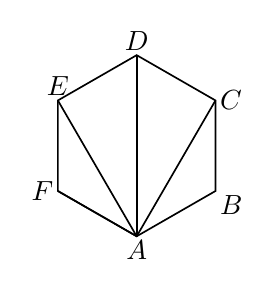
\begin{tikzpicture}[scale=1.15, semithick, every node/.style={inner sep=1.4pt}]
  \coordinate (A) at (0.00,-1.00);
  \coordinate (B) at (0.87,-0.50);
  \coordinate (C) at (0.87,0.50);
  \coordinate (D) at (0.00,1.00);
  \coordinate (E) at (-0.87,0.50);
  \coordinate (F) at (-0.87,-0.50);

  \draw (A) -- (B) -- (C) -- (D) -- (E) -- (F) -- cycle;
  \draw (A) -- (C);
  \draw (A) -- (D);
  \draw (A) -- (E);
  \draw (A) -- (F);

  \node[below] at (A) {$A$};
  \node[below right] at (B) {$B$};
  \node[right] at (C) {$C$};
  \node[above] at (D) {$D$};
  \node[above] at (E) {$E$};
  \node[left] at (F) {$F$};
\end{tikzpicture}
\end{center}
\nopagebreak[4]
\end{question}
\gkpart{三、解答题}

\begin{question}
\gkti{17}已知 $\tan\alpha=-\dfrac13$，$\cos\beta=\dfrac{\sqrt5}5$，$\alpha$，$\beta\in(0,\pi)$。

（1）求 $\tan(\alpha+\beta)$ 的值；

（2）求函数 $f(x)=\sqrt2\sin(x-\alpha)+\cos(x+\beta)$ 的最大值。

\end{question}
\begin{question}
\gkti{18}因冰雪灾害，某柑桔基地果林严重受损，为此有关专家提出一种拯救果树的方案，该方案需分两年实施且相互独立。该方案预计第一年可以使柑桔产量恢复到灾前的 $1.0$ 倍、$0.9$ 倍、$0.8$ 倍的概率分别是 $0.2$、$0.4$、$0.4$；第二年可以使柑桔产量为第一年产量的 $1.5$ 倍、$1.25$ 倍、$1.0$ 倍的概率分别是 $0.3$、$0.3$、$0.4$。

（1）求两年后柑桔产量恰好达到灾前产量的概率；

（2）求两年后柑桔产量超过灾前产量的概率。

\end{question}
\begin{question}
\gkti{19}等差数列 $\{a_n\}$ 各项均为正整数，$a_1=3$，前 $n$ 项和为 $S_n$，等比数列 $\{b_n\}$ 中，$b_1=1$，且 $b_2S_2=64$，$b_3S_3=960$。

（1）求 $a_n$ 与 $b_n$；

（2）求 $\dfrac1{S_1}+\dfrac1{S_2}+\cdots+\dfrac1{S_n}$。

\Needspace{0.4\textheight}
\end{question}
\begin{question}
\gkti{20}如图，正三棱锥 $O-ABC$ 的三条侧棱 $OA$、$OB$、$OC$ 两两垂直，且长度均为 $2$。$E$、$F$ 分别是 $AB$、$AC$ 的中点，$H$ 是 $EF$ 的中点，过 $EF$ 的一个平面与侧棱 $OA$、$OB$、$OC$ 或其延长线分别相交于 $A_1$、$B_1$、$C_1$，已知 $OA_1=\dfrac32$。

（1）证明：$B_1C_1\perp$ 平面 $OAH$；

（2）求二面角 $O-A_1B_1-C_1$ 的大小。
\nopagebreak[4]
\begin{center}% 2008 年江西卷文科第 20 题：正三棱锥 O-ABC，OA、OB、OC 两两垂直且长为 2；
%   E、F 为 AB、AC 中点，H 为 EF 中点；过 EF 的平面与 OA、OB、OC 的延长线交于 A1、B1、C1。
% 来源 PDF：gaokaomath-src/普通高考/2008/2008江西文.pdf
% SHA-256：8505b08b95152dbb1421e3f2d72c379b24c8ab6cb47bcc1dbdc8feb058459cda
% 原页：2008江西文.pdf 第 2 页（A3 三栏）第 1 栏，书页码 462。
% 绘制依据：按原页斜投影：O 在上，A 在左、B 在下、C 在右；A1 在 OA 延长线上、C1 在 OC 延长线上、
%   B1 在 OB 延长线上；截面三角形 A1B1C1 为实线，EF 与 H 在内部（虚线）。
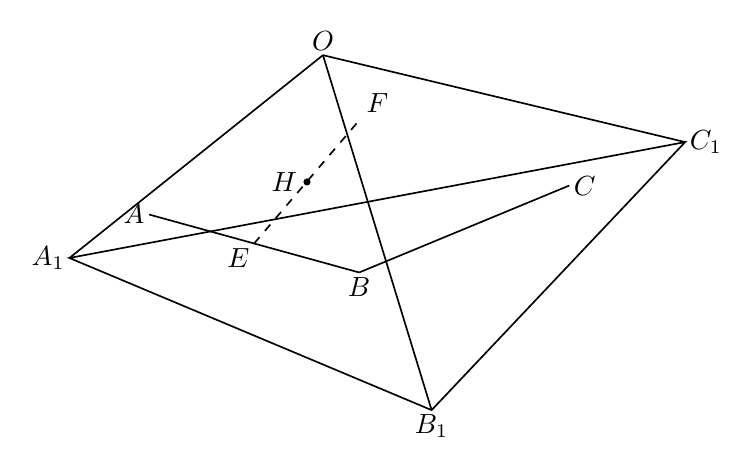
\begin{tikzpicture}[scale=0.92, semithick, every node/.style={inner sep=1.4pt}]
  \coordinate (O) at (2.60,4.30);
  \coordinate (A) at (0.20,2.10);
  \coordinate (B) at (3.10,1.30);
  \coordinate (C) at (6.00,2.50);
  \coordinate (A1) at (-0.90,1.50);
  \coordinate (B1) at (4.10,-0.60);
  \coordinate (C1) at (7.60,3.10);
  \coordinate (E) at (1.65,1.70);
  \coordinate (F) at (3.10,3.40);
  \coordinate (H) at (2.38,2.55);

  % 侧棱（延长后到 A1、B1、C1）
  \draw (O) -- (A1);
  \draw (O) -- (C1);
  \draw (O) -- (B1);

  % 截面三角形
  \draw (A1) -- (B1) -- (C1) -- cycle;

  % 底边
  \draw (A) -- (B);
  \draw (B) -- (C);

  % EF 与 H
  \draw[dashed] (E) -- (F);
  \fill (H) circle (1.4pt);

  \node[above] at (O) {$O$};
  \node[left] at (A) {$A$};
  \node[below] at (B) {$B$};
  \node[right] at (C) {$C$};
  \node[left] at (A1) {$A_1$};
  \node[below] at (B1) {$B_1$};
  \node[right] at (C1) {$C_1$};
  \node[below left] at (E) {$E$};
  \node[above right=1pt] at (F) {$F$};
  \node[left=2pt] at (H) {$H$};
\end{tikzpicture}
\end{center}
\nopagebreak[4]
\end{question}
\begin{question}
\gkti{21}已知函数 $f(x)=\dfrac14x^4+\dfrac13ax^3-a^2x^2+a^4$（$a>0$）。

（1）求函数 $y=f(x)$ 的单调区间；

（2）若函数 $y=f(x)$ 的图象与直线 $y=1$ 恰有两个交点，求 $a$ 的取值范围。

\Needspace{0.4\textheight}
\end{question}
\begin{question}
\gkti{22}已知抛物线 $y=x^2$ 和三个点 $M(x_0,y_0)$、$P(0,y_0)$、$N(-x_0,y_0)$（$y_0\neq x_0^2$，$y_0>0$），过点 $M$ 的一条直线交抛物线于 $A$、$B$ 两点，$AP$、$BP$ 的延长线分别交曲线 $C$ 于 $E$、$F$。

（1）证明 $E$、$F$、$N$ 三点共线；

（2）如果 $A$、$B$、$M$、$N$ 四点共线，问：是否存在 $y_0$，使以线段 $AB$ 为直径的圆与抛物线有异于 $A$、$B$ 的交点？如果存在，求出 $y_0$ 的取值范围，并求出该交点到直线 $AB$ 的距离；若不存在，请说明理由。
\nopagebreak[4]
\begin{center}% 2008 年江西卷文科第 22 题：抛物线 y=x^2 与三点 M(x0,y0)、P(0,y0)、N(-x0,y0)；
%   过 M 的直线交抛物线于 A、B，AP、BP 的延长线交抛物线于 E、F。
% 来源 PDF：gaokaomath-src/普通高考/2008/2008江西文.pdf
% SHA-256：8505b08b95152dbb1421e3f2d72c379b24c8ab6cb47bcc1dbdc8feb058459cda
% 原页：2008江西文.pdf 第 2 页（A3 三栏）第 3 栏，书页码 462。
% 绘制依据：按原页：抛物线开口向上，A 在左上、B 在右、M 在 B 上方偏右、P 在 y 轴上、
%   N 在 y 轴左侧；A—M—B 为割线，A—P—E 与 B—P—F 为两条直线，N—F—E—M 虚线为共线迹。
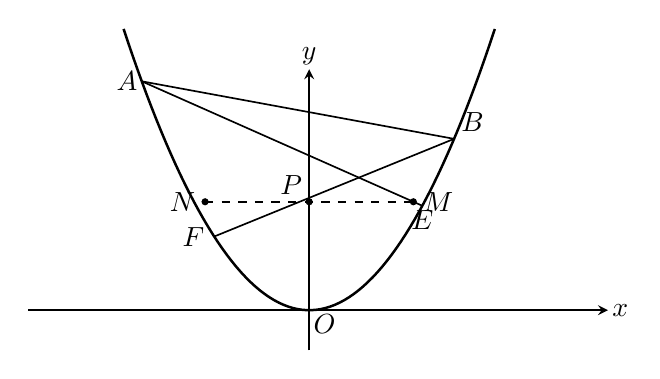
\begin{tikzpicture}[x=1.15cm, y=0.85cm, semithick, every node/.style={inner sep=1.3pt}]
  \draw[->,>=stealth] (-3.1,0) -- (3.3,0) node[right] {$x$};
  \draw[->,>=stealth] (0,-0.6) -- (0,3.6) node[above] {$y$};
  \node[below right] at (0,0) {$O$};

  \draw[line width=0.9pt, domain=-2.05:2.05, samples=80] plot (\x, {\x*\x});

  \coordinate (A) at (-1.85,3.42);
  \coordinate (M) at (1.15,1.62);
  \coordinate (B) at (1.60,2.56);
  \coordinate (P) at (0,1.62);
  \coordinate (N) at (-1.15,1.62);
  \coordinate (E) at (1.25,1.56);
  \coordinate (F) at (-1.05,1.10);

  \draw (A) -- (B);
  \draw (A) -- (E);
  \draw (B) -- (F);
  \draw[dashed] (N) -- (M);

  \fill (P) circle (1.3pt);
  \fill (M) circle (1.3pt);
  \fill (N) circle (1.3pt);

  \node[left] at (A) {$A$};
  \node[above right=1pt] at (B) {$B$};
  \node[right=2pt] at (M) {$M$};
  \node[above left=1pt] at (P) {$P$};
  \node[left=2pt] at (N) {$N$};
  \node[below] at (E) {$E$};
  \node[left=2pt] at (F) {$F$};
\end{tikzpicture}
\end{center}
\nopagebreak[4]

\end{question}